\documentclass[conference,a4paper]{IEEEtran}

\usepackage[T1]{fontenc}
\usepackage[utf8]{inputenc}
\usepackage[english]{babel}
\usepackage{newtxtext,newtxmath}
\usepackage{microtype}
\usepackage{amsmath}
\usepackage{graphicx}
\usepackage{float}
\usepackage{booktabs}
\usepackage{multirow}
\usepackage{xcolor}
\usepackage{tikz}
\usetikzlibrary{positioning,arrows.meta,fit,calc}
\usepackage{fontawesome5}
\usepackage{pgfplots}
\pgfplotsset{compat=1.18}
\usepackage[autostyle]{csquotes}
\usepackage{url}
\usepackage[hidelinks]{hyperref}
\usepackage[capitalise,nameinlink]{cleveref}
\crefname{equation}{Eq.}{Eqs.}
\Crefname{equation}{Eq.}{Eqs.}

% Let more floats share a page with text.
\renewcommand{\topfraction}{0.9}
\renewcommand{\dbltopfraction}{0.9}
\renewcommand{\textfraction}{0.1}
\renewcommand{\floatpagefraction}{0.8}
\renewcommand{\dblfloatpagefraction}{0.8}
\setcounter{topnumber}{3}
\setcounter{dbltopnumber}{2}

\graphicspath{{figures/}{../figures/}}
\renewcommand{\IEEEkeywordsname}{Keywords}

\newcommand{\Ffeat}{\mathbf{F}}
\newcommand{\film}{\mathrm{FiLM}}

\begin{document}

\title{Text-Guided Object Segmentation on Frozen\\CLIP Features with RGB-D Lifting to 3D}

% TODO: check faculty
\author{\IEEEauthorblockN{Asen Popov}
\IEEEauthorblockA{\textit{Faculty of Computer Systems and Technologies}\\
\textit{Technical University of Sofia}\\
Sofia, Bulgaria\\
asepopov@tu-sofia.bg}}

\maketitle

\begin{abstract}
A robot that is told \enquote{pick up the cup on the left} must first find the pixels and then the
3D points that the sentence refers to. This paper examines how far a small trainable decoder on top
of a \emph{frozen} CLIP encoder can go on this referring-segmentation problem. The predicted masks are
lifted into a world-frame point cloud with a calibrated RGB-D camera. Only the decoder is trained:
1.05\,M parameters, 0.7\% of the 151\,M in the full model, while the 150\,M-parameter CLIP encoders
stay frozen and their features are computed once. Trained on fewer than 4,000 sentences, text
conditioning via FiLM raises test mIoU from 0.281 (image-only) to 0.393, on par with CLIPSeg (0.385),
which uses the same frozen CLIP with a decoder of similar size trained on a far larger dataset. The two models have complementary strengths: the proposed decoder
on spatial references, CLIPSeg on object names and attributes.
\end{abstract}

\begin{IEEEkeywords}
CLIP, FiLM, point clouds, referring image segmentation, RGB-D back-projection
\end{IEEEkeywords}

% ---------------------------------------------------------------------------
\section{Introduction}
\label{sec:introduction}

Robots in homes and warehouses are increasingly instructed in natural language. Before a
manipulator can act on \enquote{the white armchair} or \enquote{the woman in the middle}, the
perception system has to answer two geometric questions: \emph{which pixels} does the sentence refer
to, and \emph{where in space} are those pixels? The first is the task of referring image segmentation
\cite{hu2016segmentation}; the second is a classic computer graphics and vision problem of inverting
the camera projection with measured depth \cite{hartley2004mvg}.

Large vision-language models such as CLIP \cite{radford2021clip} have made the first question much
more approachable: their image and text embeddings live in a shared space and transfer to many
tasks without retraining. Fine-tuning them end to end, however, is expensive and easily overfits
small datasets. This raises the question studied in this work: \emph{can a lightweight decoder,
trained on frozen CLIP features from a small dataset, ground referring expressions well enough to
localise the referred object in 3D?}

The contributions of this work are:
\begin{itemize}[\setlength{\IEEElabelindent}{0pt}]
\item a 1.05\,M-parameter decoder that fuses multi-layer CLIP patch tokens with the sentence
  embedding through feature-wise linear modulation (FiLM) \cite{perez2018film};
\item a controlled comparison, over three seeds and on a held-out test set, of image-only, FiLM and
  concatenation fusion, of the loss function and of regularisation, including a horizontal-flip
  augmentation that also swaps the words \enquote{left} and \enquote{right};
\item a comparison against the pretrained CLIPSeg model \cite{luddecke2022clipseg}, broken down by
  sentence type;
\item a geometric module that back-projects the predicted mask from RGB-D frames into a common world
  frame, with a multi-view consistency check of the result.
\end{itemize}

% ---------------------------------------------------------------------------
\section{Related Work}
\label{sec:related}

\subsection{Vision-Language Models and Dense Prediction}

CLIP \cite{radford2021clip} trains an image encoder, here a Vision Transformer (ViT)
\cite{dosovitskiy2021vit}, and a text encoder contrastively on 400 million image-text pairs. Its
global embeddings support zero-shot classification, but segmentation needs dense, per-pixel output.
MaskCLIP \cite{zhou2022maskclip} showed that the ViT patch tokens already carry usable spatial
information without any training, and LSeg \cite{li2022lseg} trained an image encoder to match
per-pixel embeddings with CLIP text embeddings of class names. CLIPSeg \cite{luddecke2022clipseg} is
closest to the present work: it keeps CLIP frozen and adds a small transformer decoder that is conditioned
on the prompt through FiLM \cite{perez2018film}, trained on the PhraseCut dataset
\cite{wu2020phrasecut}. It serves here as an external reference point.

\subsection{Referring Image Segmentation}

Referring segmentation \cite{hu2016segmentation} predicts the mask of the one object that a sentence
describes, which may need attributes (\enquote{girl in pink}), relations or position
(\enquote{man on far left}). The standard benchmarks RefCOCO and RefCOCO+ \cite{kazemzadeh2014referitgame,
yu2016refcoco} are built on COCO images \cite{lin2014coco}. State-of-the-art models such as CRIS
\cite{wang2022cris} and LAVT \cite{yang2022lavt} fine-tune large encoders with cross-modal attention
on tens of thousands of images. This work deliberately targets a much smaller regime: a frozen
encoder, a decoder of about one million parameters and fewer than one thousand training images.

\subsection{Language-Conditioned Perception in 3D}

In robotics, CLIPort \cite{shridhar2021cliport} combines CLIP semantics with spatial pathways for
tabletop manipulation. OpenScene \cite{peng2023openscene}, ConceptFusion
\cite{jatavallabhula2023conceptfusion} and LERF \cite{kerr2023lerf} attach CLIP features to 3D point
clouds, fused maps or radiance fields, so that a scene can be queried with text. These systems
build a full 3D representation first. Here, the simpler and cheaper route is taken: segmentation is
performed in 2D and only the selected pixels are lifted with the pinhole model \cite{hartley2004mvg}, using
Open3D \cite{zhou2018open3d}.

% ---------------------------------------------------------------------------
\section{Problem Formulation}
\label{sec:problem}

Given an RGB image $I \in [0,255]^{H\times W\times 3}$ and a referring sentence $t$, the goal is a
binary mask $M \in \{0,1\}^{H\times W}$ of the object that $t$ describes. The model outputs a
probability map $P(u,v) = p(\text{target} \mid I, t)$, which is thresholded at $0.5$. For a sample
with ground truth $G$, the following metrics are computed
\begin{equation}
\mathrm{IoU} = \frac{|M \cap G|}{|M \cup G|}, \qquad
\mathrm{Dice} = \frac{2\,|M \cap G|}{|M| + |G|},
\label{eq:metrics}
\end{equation}
on a $224\times 224$ grid. The mean over sentences is reported (mIoU, mean Dice) and P@0.5, the share
of sentences with $\mathrm{IoU} > 0.5$, which can be read as \enquote{the object was found}.

If, in addition, a depth map $D$, the camera intrinsics $K$ and the camera pose $T_{wc}$ are known,
the second goal is the set of 3D world points of the target, its centroid and its bounding box.

% ---------------------------------------------------------------------------
\section{Method}
\label{sec:method}

\begin{figure*}[t]
\centering
\resizebox{\textwidth}{!}{% Pipeline overview (Figure 1). Included from main.tex.
\begin{tikzpicture}[
  font=\footnotesize,
  >={Stealth[length=1.8mm]},
  arr/.style={->, thick, black!70},
  lbl/.style={font=\scriptsize, text=black!75, align=center},
  thumb/.style={inner sep=0pt, draw=black!40, line width=0.4pt}]

  % colours
  \colorlet{frozenC}{blue!55!cyan}
  \colorlet{trainC}{orange!85!red}
  \colorlet{geoC}{green!50!black}

  % encoder: trapezium narrowing to the right
  \newcommand{\encoder}[3]{% centre, name, text
    \fill[frozenC!15, draw=frozenC, line width=0.6pt, rounded corners=1.5pt]
      ($#1+(-0.65,0.75)$) -- ($#1+(0.65,0.45)$) -- ($#1+(0.65,-0.45)$) -- ($#1+(-0.65,-0.75)$) -- cycle;
    \node[lbl, text=frozenC!60!black] (#2) at #1 {#3};
    \node[text=frozenC, font=\small] at ($#1+(0,1.0)$) {\faSnowflake};}

  % ---------------- image branch ----------------
  \node[thumb, anchor=center] (rgb) at (0,0) {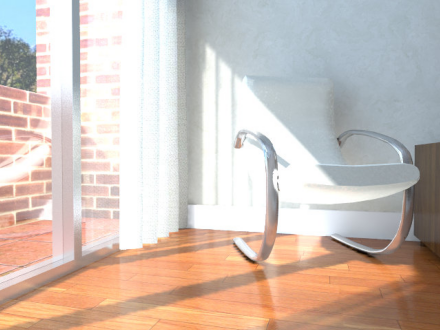
\includegraphics[width=2.1cm]{fig1_rgb.png}};
  \node[lbl, below=1mm of rgb] {RGB image};

  \encoder{(2.75,0)}{ienc}{Image\\encoder}

  % multi-layer patch tokens: four stacked grids
  \begin{scope}[shift={(4.55,-0.55)}]
    \foreach \k/\c in {3/frozenC!20, 2/frozenC!35, 1/frozenC!50, 0/frozenC!65} {
      \begin{scope}[shift={(0.13*\k,0.13*\k)}]
        \fill[\c, draw=frozenC!70!black, line width=0.4pt] (0,0) rectangle (0.9,0.9);
        \draw[white, line width=0.25pt, step=0.15] (0,0) grid (0.9,0.9);
      \end{scope}
    }
  \end{scope}
  \coordinate (tok) at (5.0,-0.1);
  \node[lbl] at (5.2,-0.95) {4 layers\\$14{\times}14$ tokens};

  % decoder: growing feature maps
  \foreach \s/\x/\n in {0.55/6.95/d1, 0.8/7.95/d2, 1.05/9.2/d3, 1.3/10.65/d4} {
    \node[draw=trainC!80!black, fill=trainC!25, line width=0.5pt, minimum size=\s cm,
          inner sep=0pt, rounded corners=1pt, font=\scriptsize, text=trainC!50!black] (\n) at (\x,0) {};
  }
  \draw[arr] (d1) -- (d2);
  \draw[arr] (d2) -- (d3);
  \draw[arr] (d3) -- (d4);
  \node[font=\scriptsize, text=trainC!50!black] at (d1) {$14^2$};
  \node[font=\scriptsize, text=trainC!50!black] at (d2) {$28^2$};
  \node[font=\scriptsize, text=trainC!50!black] at (d3) {$56^2$};
  \node[font=\scriptsize, text=trainC!50!black] at (d4) {$224^2$};
  \node[font=\small, text=trainC] (fire) at (8.8,1.0) {\faFire};
  \node[lbl, right=0.5mm of fire, text=trainC!70!black] {Decoder};
  \draw[trainC!60, dashed, rounded corners=3pt] (6.45,-0.95) rectangle (11.45,0.85);

  \node[thumb] (mask) at (13.1,0) {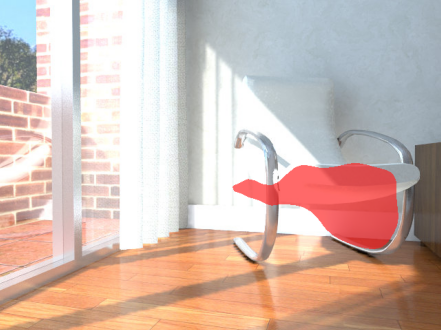
\includegraphics[width=2.1cm]{fig1_mask.png}};
  \node[lbl, below=1mm of mask] {mask $P(u,v)$};

  \node[thumb] (cloud) at (16.75,0) {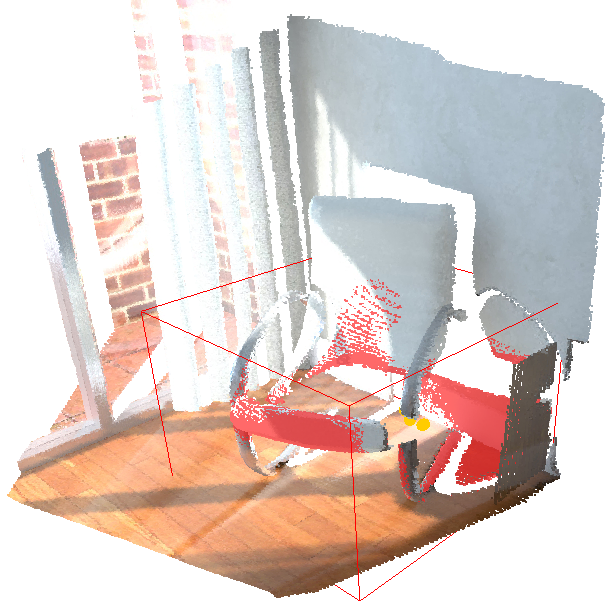
\includegraphics[width=2.0cm]{fig1_cloud.png}};
  \node[lbl, below=1mm of cloud] {3D target in world frame};

  \draw[arr] (rgb) -- (2.1,0);
  \draw[arr] (3.4,0) -- (4.5,0);
  \draw[arr] (5.95,0) -- (d1);
  \draw[arr] (d4) -- (mask);
  \draw[arr, geoC, line width=1pt] (mask.east) -- node[lbl, above, text=geoC!70!black] {lift} (cloud.west);

  % ---------------- text branch ----------------
  \node[draw=black!50, fill=black!4, rounded corners=6pt, inner sep=4pt, font=\small\itshape]
    (txt) at (0,-2.35) {\enquote{white armchair}};
  \encoder{(2.75,-2.35)}{tenc}{Text\\encoder}

  % embedding vector
  \begin{scope}[shift={(4.8,-2.35)}]
    \foreach \i in {0,...,7} \fill[frozenC!25!white!80!frozenC, draw=frozenC!70!black, line width=0.3pt]
      (-0.12,-0.6+0.15*\i) rectangle (0.12,-0.45+0.15*\i);
  \end{scope}
  \node[lbl] at (4.8,-3.15) {512-d};

  \node[circle, draw=trainC!80!black, fill=trainC!25, inner sep=1.5pt, lbl] (mlp) at (6.25,-2.35) {MLP};
  \node[lbl, text=trainC!70!black] at (7.55,-2.0) {$(\gamma,\beta)$};

  \draw[arr] (txt) -- (2.1,-2.35);
  \draw[arr] (3.4,-2.35) -- (4.6,-2.35);
  \draw[arr] (5.0,-2.35) -- (mlp);
  % FiLM into the first two decoder stages
  \draw[arr, trainC!80!black] (mlp.east) -| (d1.south |- 0,-1.25) -- (d1.south);
  \draw[arr, trainC!80!black] (mlp.east) -| (d2.south |- 0,-1.25) -- (d2.south);
  \node[lbl, text=trainC!70!black, anchor=west] at (8.35,-1.55) {FiLM: $(1+\gamma)\odot\Ffeat+\beta$};

  % ---------------- depth branch ----------------
  \node[thumb] (depth) at (14.9,-2.35) {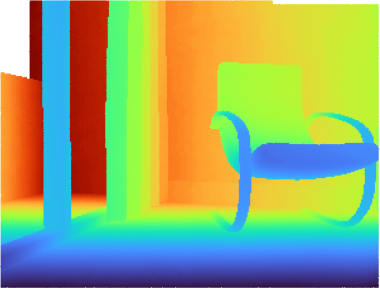
\includegraphics[width=1.7cm]{fig1_depth.png}};
  \node[lbl, right=1.5mm of depth, anchor=west] {depth $D$\\$K$, $T_{wc}$};
  \draw[arr, geoC] (depth.north) -- (14.9,-0.05);
  \node[lbl, text=geoC!70!black, anchor=north] at (14.9,-3.15) {$P_w = T_{wc}\,Z K^{-1}[u,v,1]^\top$};
\end{tikzpicture}
}
\caption{Overview of the method. \textcolor{blue!55!cyan}{\faSnowflake}~frozen CLIP encoders;
\textcolor{orange!85!red}{\faFire}~trainable decoder (1.05\,M parameters), conditioned on the sentence
through FiLM; green: lifting the mask to 3D with a calibrated RGB-D frame.}
\label{fig:pipeline}
\end{figure*}

\Cref{fig:pipeline} shows the full pipeline.

\subsection{Frozen CLIP Features}

The public \texttt{openai/clip-vit-base-patch16} model is used. An image resized to $224\times224$
gives $14\times14$ patch tokens of dimension 768 in each of the 12 transformer layers. Early layers
are more spatial and later ones more semantic, so the patch tokens of layers 3, 6, 9 and 12
are kept (the class token is dropped). The sentence is encoded by the CLIP text encoder into a 512-d
embedding $e_t$. Both encoders are frozen, so their outputs are computed once and cached, and a full
training run takes 30--40\,s on a laptop GPU.

\subsection{Text-Conditioned Decoder}

Each of the four token maps $z_\ell$ is normalised and projected to $C = 128$ channels, and the
projections are summed:
\begin{equation}
\Ffeat_0 = \sum_{\ell \in \{3,6,9,12\}} W_\ell \, \mathrm{LN}(z_\ell) \in \mathbb{R}^{14\times14\times C}.
\end{equation}
The text enters through FiLM \cite{perez2018film}: a small MLP maps $e_t$ to a per-channel scale
$\gamma$ and shift $\beta$, which modulate the feature map
\begin{equation}
\film(\Ffeat \mid t) = \bigl(1 + \gamma(e_t)\bigr) \odot \Ffeat + \beta(e_t).
\label{eq:film}
\end{equation}
The MLP is zero-initialised, so at the start of training $\gamma = \beta = 0$ and FiLM passes the
features through unchanged. FiLM is applied at two stages,
at $14\times14$ and after the first upsampling. The decoder then refines the features with
$3\times3$ convolution blocks at $14^2$, $28^2$ and $56^2$, predicts one logit per pixel with a
$1\times1$ convolution and upsamples bilinearly to $224\times224$.

As controls, the same decoder \emph{without} text (M0, image-only) is used, as well as a variant that
concatenates the broadcast text embedding to the features instead of FiLM (M1b, concat). Appending normalised $(x,y)$ coordinate channels \cite{liu2018coordconv}, which can help
convolutional networks with positional words, was also tested.

\subsection{Loss and Training}

The decoder is trained with binary cross-entropy plus soft Dice \cite{milletari2016vnet}, which
counteracts the imbalance between small objects and large backgrounds:
\begin{equation}
\mathcal{L} = \mathrm{BCE}(P, G) + \lambda \left(1 - \frac{2\sum P\,G + \epsilon}{\sum P + \sum G + \epsilon}\right),
\quad \lambda = 1.
\end{equation}
Optimisation uses AdamW \cite{loshchilov2019adamw} (learning rate $3\cdot10^{-4}$, weight decay
$0.01$), a one-cycle schedule \cite{smith2019onecycle}, batches of 32, at most 30 epochs, and early
stopping on validation mIoU.

\subsection{Language-Aware Flip Augmentation}

Horizontal flipping is the standard augmentation for segmentation, but it changes the meaning of
referring expressions: after a flip, \enquote{man on the left} is on the right. Therefore, the image
and the mask are flipped, and the words \enquote{left} and \enquote{right} are swapped in the sentence
before it is encoded. The swap affects 48\% of all sentences in the dataset, so a plain flip would produce
wrong labels for almost half of the training data. Flipped CLIP features are cached in the same way
as the originals.

\subsection{Lifting the Mask to 3D}
\label{sec:method-3d}

With an aligned depth map $D$ (in millimetres) and intrinsics
$K = \bigl[\begin{smallmatrix} f_x & 0 & c_x\\ 0 & f_y & c_y \\ 0 & 0 & 1\end{smallmatrix}\bigr]$,
the pinhole model $\lambda[u,v,1]^\top = K P_c$ is inverted for every masked pixel:
\begin{equation}
Z = \frac{D(u,v)}{1000},\quad X = \frac{(u - c_x)\,Z}{f_x},\quad Y = \frac{(v - c_y)\,Z}{f_y}.
\label{eq:backproject}
\end{equation}
Camera points are moved into the world frame with the rigid camera pose
$T_{wc} = \bigl[\begin{smallmatrix} R & \mathbf{t} \\ \mathbf{0}^\top & 1\end{smallmatrix}\bigr]$:
\begin{equation}
P_w = R\,P_c + \mathbf{t}.
\label{eq:world}
\end{equation}
Pixels without depth or beyond 4\,m are skipped. Before lifting, the mask is cleaned in 2D: connected
components smaller than 10\% of the largest are removed, and the mask is eroded by 3 pixels, because
at an object's silhouette the depth sensor often measures the background, which would create
\enquote{flying} points between object and wall. The lifted points are downsampled to a 1\,cm voxel
grid and filtered with a statistical outlier test \cite{rusu2008objectmaps}. The target is reported
by its centroid and its axis-aligned bounding box.

Open3D \cite{zhou2018open3d} is used for back-projection, transformation and rendering. Unit tests on
synthetic depth with $f_x \neq f_y$ and an off-centre principal point check that it implements
exactly \cref{eq:backproject,eq:world}, including Open3D's convention of storing the inverse pose
(world to camera) as the \enquote{extrinsic} matrix.

% ---------------------------------------------------------------------------
\section{Experimental Setup}
\label{sec:setup}

\subsection{Data}

The data come from RefCOCO-M \cite{refcocom}, a re-annotation of RefCOCO \cite{yu2016refcoco} with refined,
pixel-accurate masks: 1,190 COCO images, 2,080 object masks and 5,598 referring sentences. It is
distributed as a single split, so it was partitioned \emph{by image} (seed 0) into
train/val/test = 833/178/179 images (3,952/857/789 sentences). Splitting by image guarantees that no
test image, and no object in it, is seen during training. About two thirds of the sentences
contain spatial words (\enquote{left}, \enquote{right}, \enquote{behind}, \enquote{second}, \dots).

The 3D experiments use the Redwood RGB-D sample shipped with Open3D \cite{choi2015redwood}:
five $640\times480$ frames of a rendered living room with aligned depth, intrinsics
($f_x = f_y = 525$, $c_x = 319.5$, $c_y = 239.5$) and a camera pose per frame.

\subsection{Protocol}

Every variant is trained with three seeds; the mean and standard deviation are reported. All design
choices, including the final model, were made on the validation set. The test set was evaluated
once, after tuning had ended. CLIPSeg (\texttt{CIDAS/clipseg-rd64-refined}) is evaluated with its
own $352\times352$ input, its output is resized to the same $224\times224$ grid, and its threshold
(0.25) is chosen on validation. Because CLIPSeg was trained on different data, it is a reference
point, not a controlled baseline. Latency is measured at batch size 1 on an NVIDIA RTX 4060 Laptop GPU.

% ---------------------------------------------------------------------------
\section{Results}
\label{sec:results}

\begin{table}[!t]
\caption{Test results (789 sentences, 179 images), mean over 3 seeds. Params: trainable parameters on top of the same frozen CLIP ViT-B/16 (150\,M)}
\label{tab:results}
\centering
\footnotesize
\setlength{\tabcolsep}{4pt}
\begin{tabular}{@{}lrlll@{}}
\toprule
Model & Params & mIoU & Dice & P@0.5 \\
\midrule
M0 image-only            & 0.66\,M & $0.281 \pm 0.002$ & 0.397 & 0.179 \\
M1b concat               & 0.85\,M & $0.353 \pm 0.012$ & 0.456 & 0.341 \\
M1 FiLM                  & 1.05\,M & $0.375 \pm 0.013$ & 0.478 & 0.375 \\
\quad no coord.\ channels & 1.05\,M & $0.375 \pm 0.005$ & 0.478 & 0.381 \\
\quad BCE only           & 1.05\,M & $0.332 \pm 0.009$ & 0.428 & 0.319 \\
\midrule
R1: + dropout, wd        & 1.05\,M & $0.392 \pm 0.013$ & 0.495 & 0.398 \\
\textbf{R2: + flip (final)} & 1.05\,M & $\mathbf{0.393 \pm 0.013}$ & \textbf{0.498} & \textbf{0.400} \\
R3: R1 + R2              & 1.05\,M & $0.403 \pm 0.012$ & 0.506 & 0.414 \\
\midrule
CLIPSeg$^{*}$ \cite{luddecke2022clipseg} & 1.13\,M & $0.385$ & 0.492 & 0.371 \\
\bottomrule
\multicolumn{5}{@{}l}{\scriptsize $^{*}$Trained by its authors on PhraseCut \cite{wu2020phrasecut}, used as released.}
\end{tabular}
\end{table}

\subsection{Text Conditioning and Fusion}

\Cref{tab:results} summarises the test results. Text conditioning is the decisive ingredient: FiLM
improves mIoU over the image-only decoder by $+0.094 \pm 0.012$, and P@0.5 more than doubles, from
0.18 to 0.38. The image-only model can only learn \enquote{segment a salient object}, which is
sometimes right by chance. FiLM beats concatenation by $+0.021 \pm 0.004$, in all three seeds,
while concatenation uses 0.2\,M fewer parameters. Removing Dice from the loss costs $0.043$ mIoU.
Coordinate channels bring no gain, which suggests that CLIP's patch tokens already encode position
well enough; they are therefore omitted from the final model.

\Cref{fig:language} shows the effect qualitatively: on the same image the image-only model returns
the same mask for every sentence, whereas the FiLM model switches targets. On the 91 test images
with at least two described objects, the final model segments \emph{both} sentences correctly
(IoU $> 0.5$) in 19.8\% of cases; the image-only model never does.

\begin{figure*}[t]
\centering
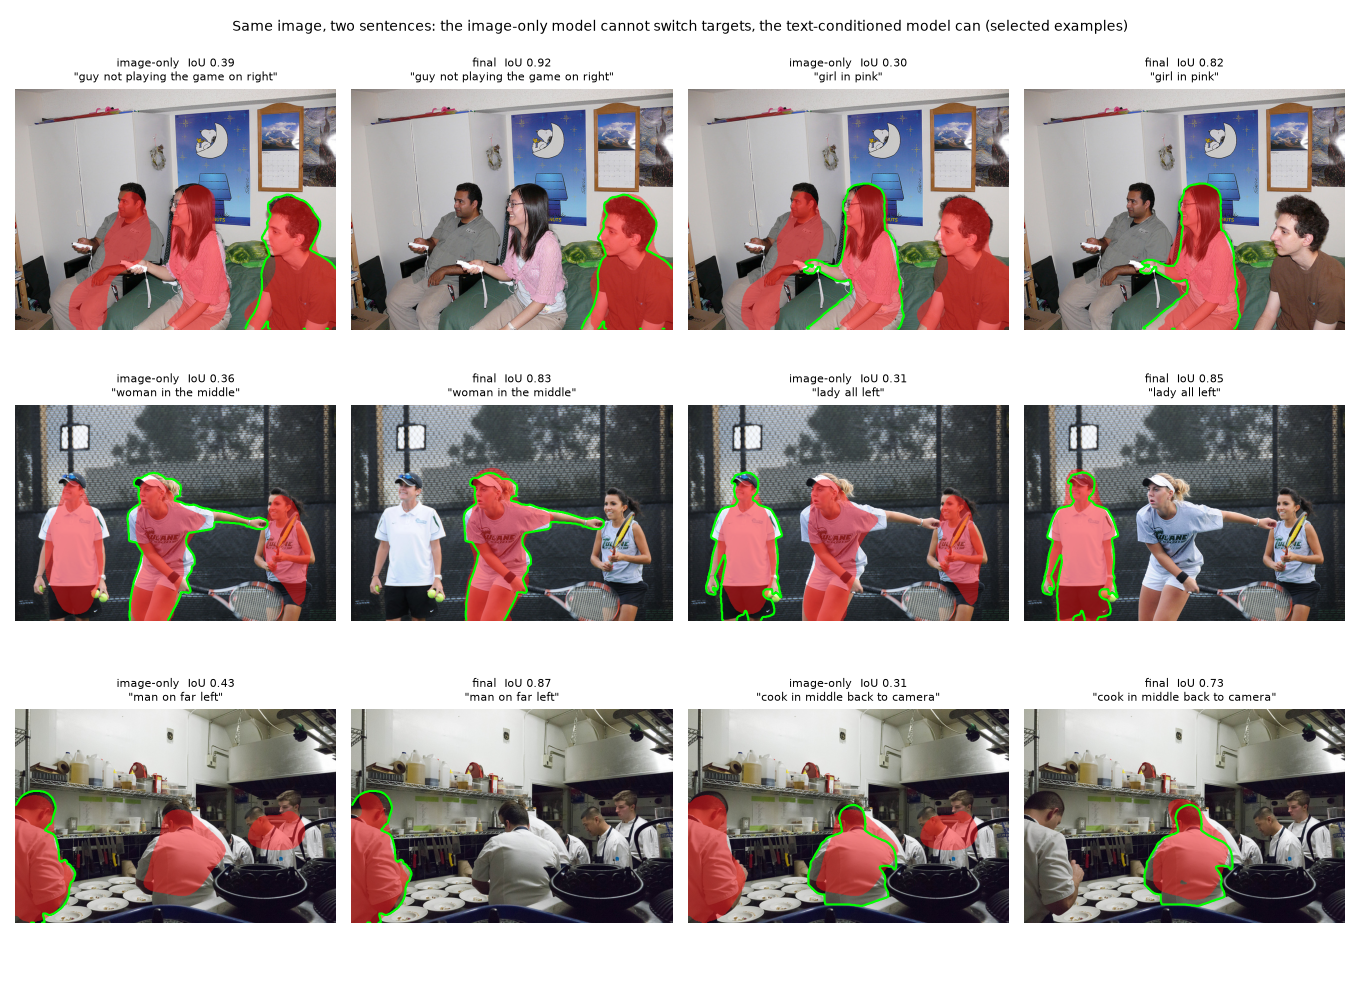
\includegraphics[width=0.92\textwidth, trim=0 228 0 40, clip]{gallery_language.png}
\caption{Same image, two sentences (test set). Columns 1 and 3: image-only decoder; columns 2 and 4:
final FiLM model. Green outline: ground truth; red: prediction. The image-only model cannot change
its answer when the sentence changes.}
\label{fig:language}
\end{figure*}

\subsection{Overfitting and Regularisation}

With fewer than a thousand training images the decoder overfits strongly. \Cref{fig:curves} shows
the classic pattern: training loss falls steadily to about 0.2, while validation loss reaches its
minimum around epochs 9--13 and then rises again, to about 0.96 at the last epoch. The FiLM model
reaches 0.76 mIoU on the training images but 0.41 on validation (\cref{fig:gap}). On validation, dropout with stronger
weight decay (R1) reduced the gap between training and validation mIoU from 0.35 to 0.32, and the language-aware flip
(R2) reduced it to 0.28 while giving the best validation mIoU (0.432 vs.\ 0.413). R2 was
therefore selected as the final model. On the test set R2 improves over the FiLM model by $+0.018$. R3,
which combines both, is numerically higher on test (0.403), but the difference from R2 is within
seed variation and it was not meaningfully better on validation (0.433 vs.\ 0.432), so the choice made
on validation is kept.

\begin{figure}[!htbp]
\centering
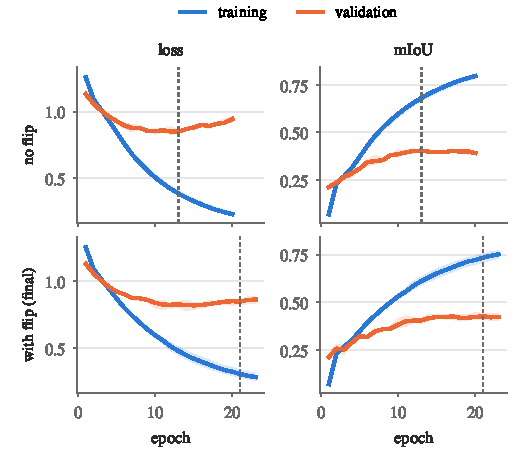
\includegraphics[width=\columnwidth]{overfitting_curves.pdf}
\caption{Learning curves of the FiLM model without (top) and with (bottom) flip augmentation, mean
of 3 runs (band: range of the runs). Training loss keeps falling while validation loss reaches its
minimum and rises again; validation mIoU stops improving after about 12 epochs. Dotted line: epoch
with the best validation mIoU. Training values are running averages during each epoch.}
\label{fig:curves}
\end{figure}

\begin{figure}[!htbp]
\centering
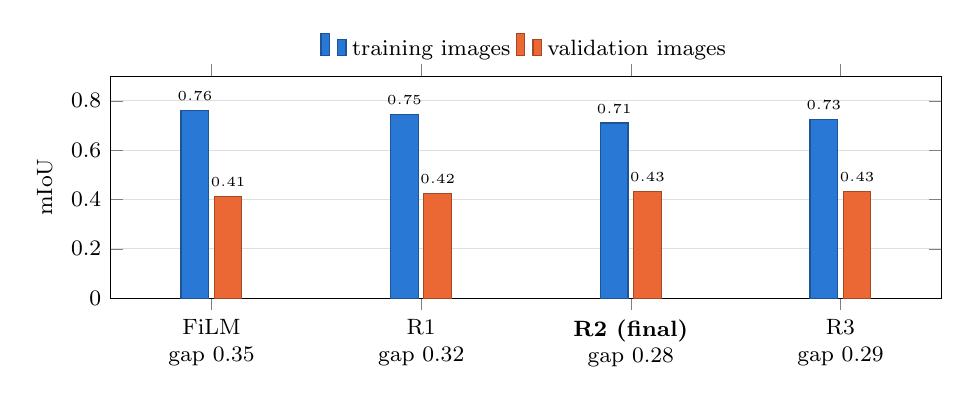
\begin{tikzpicture}
\definecolor{trainC}{HTML}{2A78D6}\definecolor{valC}{HTML}{EB6834}
\begin{axis}[
  ybar, bar width=10pt, width=\columnwidth, height=4.4cm,
  ymin=0, ymax=0.9, ylabel={mIoU}, ylabel style={font=\footnotesize},
  symbolic x coords={base, r1, r2, r3}, xtick=data,
  xticklabels={FiLM\\gap 0.35, R1\\gap 0.32, \textbf{R2 (final)}\\gap 0.28, R3\\gap 0.29},
  x tick label style={font=\footnotesize, align=center},
  y tick label style={font=\footnotesize, /pgf/number format/fixed},
  enlarge x limits=0.16,
  legend style={at={(0.5,1.02)}, anchor=south, font=\footnotesize, draw=none, fill=none, legend columns=2},
  legend cell align=left,
  nodes near coords, nodes near coords style={font=\tiny, /pgf/number format/fixed, /pgf/number format/precision=2},
  ymajorgrids, grid style={gray!25}]
\addplot[fill=trainC, draw=trainC!70!black] coordinates {(base,0.760) (r1,0.746) (r2,0.710) (r3,0.725)};
\addplot[fill=valC, draw=valC!70!black] coordinates {(base,0.413) (r1,0.424) (r2,0.432) (r3,0.433)};
\legend{training images, validation images}
\end{axis}
\end{tikzpicture}
\caption{mIoU on the training and validation images for the regularisation variants (selected
checkpoints, evaluation mode, mean of 3 runs). The gap below each pair measures overfitting.}
\label{fig:gap}
\end{figure}

\subsection{Comparison with CLIPSeg}

Overall, the final model and CLIPSeg are level (0.393 vs.\ 0.385; the difference is smaller than
the seed variation). Both use the same frozen CLIP encoders and a decoder of similar size (1.05\,M
vs.\ 1.13\,M parameters), so the comparison mainly reflects the training data: fewer than 4,000
RefCOCO-M sentences here, against the much larger PhraseCut dataset for CLIPSeg. The breakdown by sentence type in \cref{fig:breakdown} shows that the two
models are good at different things. The proposed decoder, trained on RefCOCO-style sentences, is much better
on spatial references (0.386 vs.\ 0.307). CLIPSeg, trained on the larger PhraseCut dataset, is much
better on sentences that name an object or its attributes without position (0.530 vs.\ 0.407). The
proposed model is also faster: about 5.5\,ms per image and sentence end to end, of which 4.7\,ms is CLIP and
0.8\,ms the decoder, compared with 7.7\,ms for CLIPSeg.

\begin{figure}[!htbp]
\centering
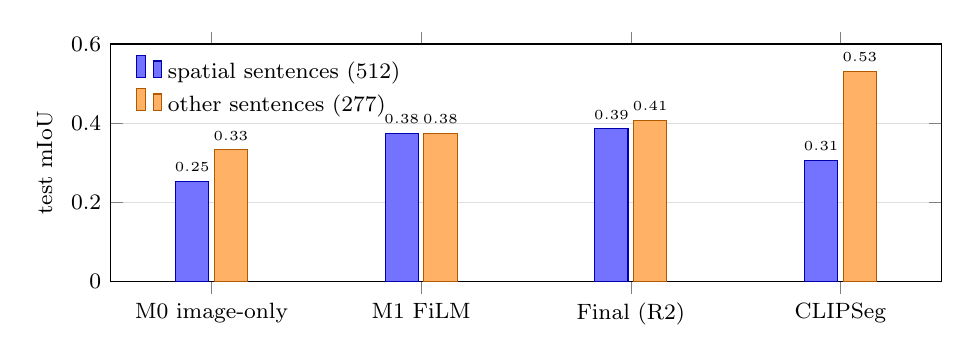
\begin{tikzpicture}
\begin{axis}[
  ybar, bar width=12pt, width=\columnwidth, height=4.6cm,
  ymin=0, ymax=0.6, ylabel={test mIoU}, ylabel style={font=\footnotesize},
  symbolic x coords={M0 image-only, M1 FiLM, Final (R2), CLIPSeg},
  xtick=data, x tick label style={font=\footnotesize},
  y tick label style={font=\footnotesize, /pgf/number format/fixed},
  enlarge x limits=0.16,
  legend style={at={(0.02,0.98)}, anchor=north west, font=\footnotesize, draw=none, fill=none},
  legend cell align=left,
  nodes near coords, nodes near coords style={font=\tiny, /pgf/number format/fixed, /pgf/number format/precision=2},
  ymajorgrids, grid style={gray!25}]
\addplot[fill=blue!55, draw=blue!70!black] coordinates
  {(M0 image-only,0.253) (M1 FiLM,0.375) (Final (R2),0.386) (CLIPSeg,0.307)};
\addplot[fill=orange!60, draw=orange!70!black] coordinates
  {(M0 image-only,0.333) (M1 FiLM,0.375) (Final (R2),0.407) (CLIPSeg,0.530)};
\legend{spatial sentences (512), other sentences (277)}
\end{axis}
\end{tikzpicture}
\caption{Test mIoU by sentence type. Spatial sentences contain words such as \enquote{left},
\enquote{right} or \enquote{behind}.}
\label{fig:breakdown}
\end{figure}

% Wide figure defined here so that it lands at the top of the page with the 3D section.
\begin{figure*}[t]
\centering
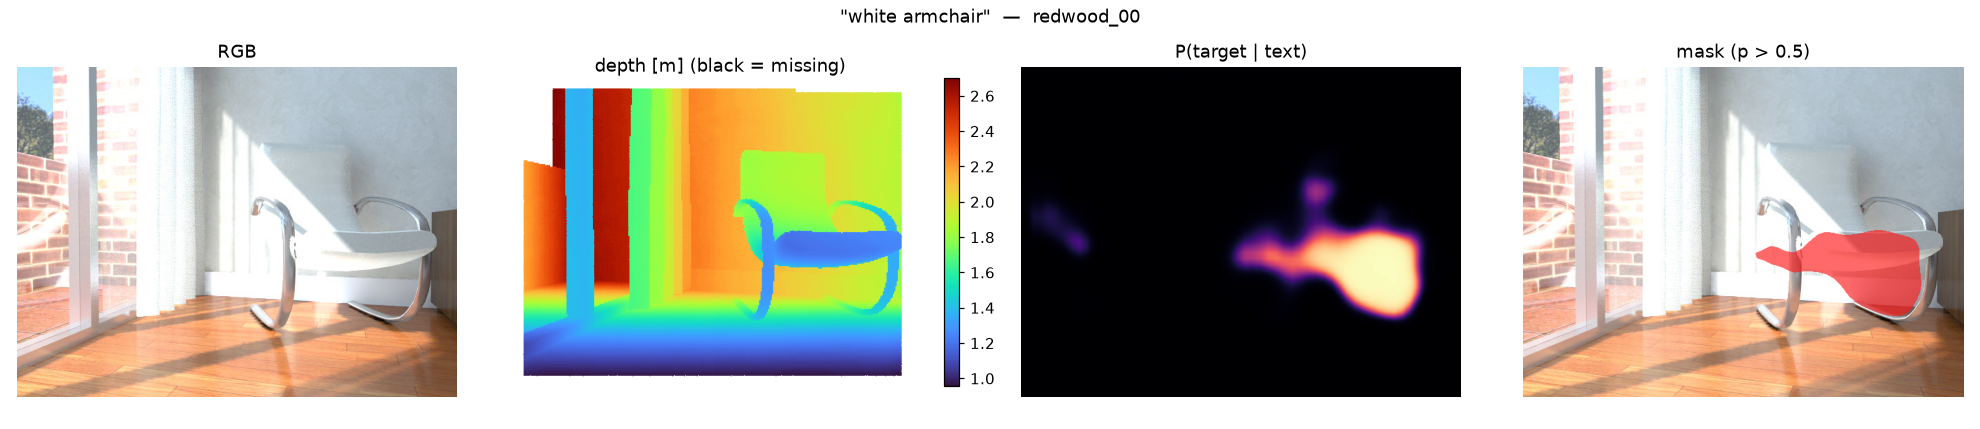
\includegraphics[width=0.95\textwidth, trim=0 0 0 30, clip]{white-armchair_redwood_00_2d.png}
\caption{\enquote{white armchair} on Redwood frame 0: RGB, measured depth, predicted probability
map and thresholded mask. The mask mainly covers the seat; the thin metal frame is missed.}
\label{fig:redwood2d}
\end{figure*}

\subsection{Failure Cases}

The hardest sentences are those that hinge on colour or clothing (\enquote{girl in pink},
\enquote{man in white shirt}): 0.320 mIoU against 0.419 for the rest, which is consistent with
CLIPSeg's advantage on attributes. Crowded images with four or more annotated objects are also
difficult (0.233 mIoU), mostly because the model picks the right kind of object but the wrong
instance. Finally, the decoder predicts at $56\times56$, so thin structures and exact boundaries are
lost.

\subsection{3D Localisation}

\Cref{fig:redwood2d,fig:redwood3d} show the geometric module on the Redwood sequence for the
sentence \enquote{white armchair}. The predicted mask is lifted from each of the five frames into the
common world frame. Because the chair is static, its centroid should land at the same world point
from every viewpoint; the measured spread is 3.0\,cm on average and 4.4\,cm at most (4.4\,cm /
5.2\,cm without flip augmentation). The five scene clouds overlap without visible double contours,
so the remaining spread is caused by the masks covering slightly different parts of the chair, not
by pose errors.

\begin{figure}[!htbp]
\centering
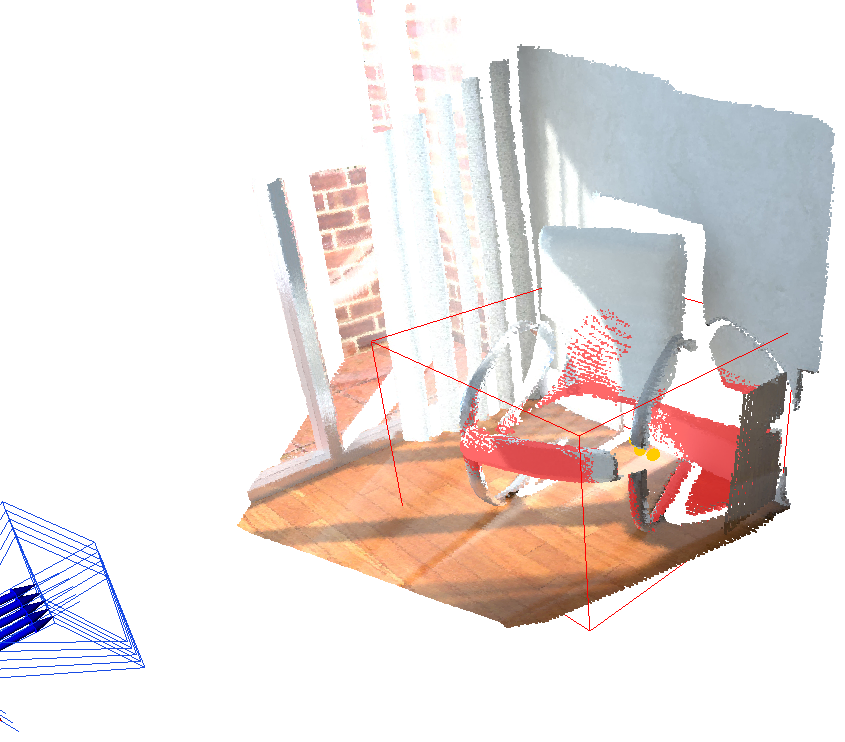
\includegraphics[width=0.85\columnwidth]{white-armchair_3d_crop.png}
\caption{World-frame point cloud fused from five RGB-D frames. Red: target points; yellow: per-frame
centroids; red box: fused bounding box; blue: camera frustums.}
\label{fig:redwood3d}
\end{figure}

The 3D results also expose the limits of the 2D model. Redwood is a synthetic render and differs
from COCO photographs, so the mask mainly covers the seat cushion and the bounding box
underestimates the chair's height. Sentences about background regions (\enquote{the window},
\enquote{the floor}) fail: RefCOCO only annotates discrete objects, so the model has learned that
the answer is always an object and falls back to the most salient one.

% ---------------------------------------------------------------------------
\section{Limitations and Future Work}
\label{sec:limitations}

The main limitation is the amount of training data. RefCOCO-M contains refined masks for the
RefCOCO \emph{evaluation} images, and 833 training images leave a gap of 0.28 between training and validation mIoU
even with augmentation. Training on the original RefCOCO training split (about 17k images, disjoint
from the images used here) is the natural next step. The reported numbers come from a custom split and are not comparable
with published RefCOCO benchmarks. CLIP and CLIPSeg may also have seen COCO images during
pre-training. On the geometric side, each frame only sees visible surfaces, the bounding box is
axis-aligned rather than oriented, and the 3D output is a localisation, not a grasp or manipulation
plan. Higher-resolution decoding, oriented boxes and fusion of the per-frame masks into one
volumetric map are straightforward extensions.

% ---------------------------------------------------------------------------
\section{Conclusion}
\label{sec:conclusion}

A decoder with about one million parameters on frozen CLIP features can ground referring
expressions: text conditioning through FiLM improves test mIoU from 0.281 to 0.393, matches the
pretrained CLIPSeg model overall and clearly outperforms it on spatial references. A language-aware
flip augmentation, which swaps \enquote{left} and \enquote{right}, is a cheap and effective
regulariser for this task. Combined with the pinhole model and a calibrated RGB-D camera, the 2D
masks become consistent 3D localisations within a few centimetres across viewpoints, a first step
from \enquote{what the user said} to \enquote{where the robot should look}.

\section*{Code Availability}

Code, data split and scripts for all results:
\url{https://github.com/Apsie09/Text-Guided-Segmentation-3D}.

\bibliographystyle{IEEEtran}
\bibliography{refs}

\end{document}
